%---------------------------------------
% The CGEM Poster Beamer template
%
%---------------------------------------
% About:
% The poster template is a simple
% wrapper around the Beamer Poster
% package for CGEM style work.
%
%---------------------------------------
% Author:
% R. Nate Crummett
%
%---------------------------------------
\documentclass[dark]{cgem-poster}

% Bibliography folder path
\bibliographypath{Bib}

% Paths to images
\graphicspath{{Fig/}{Logo/}}

%---------------------------------------
% Poster specific macros
\newcommand{\PosterTitle}{Poster Title --- Yaoguo Doesn't Like Corny}
\newcommand{\PosterFirstAuthor}{R. Nate Crummett}
\newcommand{\PosterFirstAuthorContact}{robert\_crummett@mines.edu}
\newcommand{\PosterSecondAuthor}{Yaoguo Li}
\newcommand{\PosterAffiliationCGEM}{Center for Gravity, Electrical \& Magnetic Studies}
\newcommand{\PosterAffiliationMines}{Colorado School of Mines}
\newcommand{\PosterAffiliationGeophysics}{Department of Geophysics}

%---------------------------------------
% Poster
\colorlet{PosterSubtitleColor}{ZeroColor!50}
\colorlet{PosterBackgroundColor}{ZeroColor!80}

\begin{document}

%---------------------------------------
% BEGIN POSTER TITLE SECTION

% Title parameters
\newcommand{\titleheight}{0.09\pageheight}
\newcommand{\PosterCGEMLogoHeight}{\dimexpr(\titleheight - 12mm)\relax}

% Title background block
\begin{textblock*}{\pagewidth}(0cm,0cm)
  \textblockcolor{ZeroColor}
  \begin{minipage}[t][\titleheight{}][t]{\pagewidth}
  \end{minipage}
\end{textblock*}

% Title text and text background color
\begin{textblock*}{0.85\pagewidth}(0.075\pagewidth,0cm)
  \textblockcolor{ZeroColor}
  \begin{center}
    \vspace{5mm}
    % Poster title
    \Large
    \textbf{
      \PosterTitle{}
    }
    \par
    \vspace{5mm}
    % Poster authors and affilitations
    \normalsize
    { \color{PosterSubtitleColor}
    \PosterFirstAuthor{}* \& \PosterSecondAuthor{}
    \par
    \small
    \PosterAffiliationCGEM{} --- \PosterAffiliationGeophysics{} --- \PosterAffiliationMines{}
    }
  \end{center}
\end{textblock*}

% Mines logo
\begin{textblock*}{\titleheight{}}(0.01\pagewidth,0cm)
  \textblockcolor{ZeroColor}
  \centering
  \hspace*{-20.72449pt}
  \includegraphics[height=\titleheight{}]{\LogoFileMines}
\end{textblock*}

% CGEM logo
\begin{textblock*}{\titleheight{}}(0.92\pagewidth,5mm)
  \textblockcolor{ZeroColor}
  \centering
  \includegraphics[height=\PosterCGEMLogoHeight{}]{\LogoFileCGEM}
\end{textblock*}

% Contact information
\begin{textblock*}{0.2\pagewidth}(0.869\pagewidth,0.991\pageheight)
  \textblockcolor{ZeroColor}
  \tiny
  { \color{PosterBackgroundColor}
  *Contact: \PosterFirstAuthorContact{}
  }
\end{textblock*}

% END POSTER TITLE SECTION
%---------------------------------------
% BEGIN POSTER BACKGROUND SECTION

% Poster outer margin dimensions
\newlength{\PosterOuterMarginSize}
\setlength{\PosterOuterMarginSize}{7.5mm}

\newcommand{\PosterBackgroundLeft}{\PosterOuterMarginSize}
\newcommand{\PosterBackgroundWidth}{\dimexpr (\pagewidth - 2\PosterOuterMarginSize)\relax}
\newcommand{\PosterBackgroundTop}{\dimexpr (\titleheight + \PosterOuterMarginSize)\relax}
\newcommand{\PosterBackgroundHeight}{\dimexpr (\pageheight - \PosterBackgroundTop - \PosterOuterMarginSize)\relax}

% Outer margin
\begin{textblock*}{\PosterBackgroundWidth{}}(\PosterBackgroundLeft{},\PosterBackgroundTop{})
  \textblockcolor{PosterBackgroundColor}
  \begin{minipage}[t][\PosterBackgroundHeight{}][t]{\PosterBackgroundWidth{}}
  \end{minipage}
\end{textblock*}

% Poster inner content dimensions
\newlength{\PosterInnerMarginSize}
\setlength{\PosterInnerMarginSize}{1cm}

\newcommand{\PosterInnerLeft}{\dimexpr (\PosterOuterMarginSize + \PosterInnerMarginSize)\relax}
\newcommand{\PosterInnerWidth}{\dimexpr (\PosterBackgroundWidth - 2\PosterInnerMarginSize)\relax}
\newcommand{\PosterInnerTop}{\dimexpr (\PosterBackgroundTop + \PosterInnerMarginSize)\relax}
\newcommand{\PosterInnerHeight}{\dimexpr (\PosterBackgroundHeight - 2\PosterInnerMarginSize)\relax}

% Break content into three columns for example
\newcommand{\PosterColumnWidth}{\dimexpr ((\PosterInnerWidth - 2\PosterInnerMarginSize)/3)\relax}

% Column one dimensions
\newcommand{\PosterColumnOneLeft}{\PosterInnerLeft}
\newcommand{\PosterColumnOneWidth}{\PosterColumnWidth}
\newcommand{\PosterColumnOneTop}{\PosterInnerTop}
\newcommand{\PosterColumnOneHeight}{\PosterInnerHeight}

% Column one background
\begin{textblock*}{\PosterColumnOneWidth{}}(\PosterColumnOneLeft{},\PosterColumnOneTop{})
  \textblockcolor{ZeroColor}
  \begin{minipage}[t][\PosterColumnOneHeight{}][t]{\PosterColumnOneWidth{}}
  \end{minipage}
\end{textblock*}

% Column two dimensions
\newcommand{\PosterColumnTwoLeft}{\dimexpr (\PosterColumnOneLeft + \PosterColumnOneWidth + \PosterInnerMarginSize)\relax}
\newcommand{\PosterColumnTwoWidth}{\PosterColumnWidth}
\newcommand{\PosterColumnTwoTop}{\PosterInnerTop}
\newcommand{\PosterColumnTwoHeight}{\PosterInnerHeight}

% Column two background
\begin{textblock*}{\PosterColumnTwoWidth{}}(\PosterColumnTwoLeft{},\PosterColumnTwoTop{})
  \textblockcolor{ZeroColor}
  \begin{minipage}[t][\PosterColumnTwoHeight{}][t]{\PosterColumnTwoWidth{}}
  \end{minipage}
\end{textblock*}

% Column three dimensions
\newcommand{\PosterColumnThreeLeft}{\dimexpr (\PosterColumnTwoLeft + \PosterColumnTwoWidth + \PosterInnerMarginSize)\relax}
\newcommand{\PosterColumnThreeWidth}{\PosterColumnWidth}
\newcommand{\PosterColumnThreeTop}{\PosterInnerTop}
\newcommand{\PosterColumnThreeHeight}{\PosterInnerHeight}

% Column three background 
\begin{textblock*}{\PosterColumnThreeWidth{}}(\PosterColumnThreeLeft{},\PosterColumnThreeTop{})
  \textblockcolor{ZeroColor}
  \begin{minipage}[t][\PosterColumnThreeHeight{}][t]{\PosterColumnThreeWidth{}}
  \end{minipage}
\end{textblock*}

% Horizontal bar
\newcommand{\PosterColumnHorizontalBar}{ \textcolor{PosterBackgroundColor}{\noindent\makebox[\linewidth]{\rule{1.01\PosterColumnWidth}{\PosterInnerMarginSize}}} }

% END POSTER BACKGROUND SECTION
%---------------------------------------
% BEGIN POSTER CONTENT SECTION

\newlength{\PosterTextMarginSize}
\setlength{\PosterTextMarginSize}{1cm}

% Column one text block dimensions
\newcommand{\PosterColumnOneTextLeft}{\dimexpr (\PosterColumnOneLeft + \PosterTextMarginSize)\relax}
\newcommand{\PosterColumnOneTextWidth}{\dimexpr (\PosterColumnOneWidth - 2\PosterTextMarginSize)\relax}
\newcommand{\PosterColumnOneTextTop}{\dimexpr (\PosterColumnOneTop + \PosterTextMarginSize)\relax}
\newcommand{\PosterColumnOneTextHeight}{\dimexpr (\PosterColumnOneHeight - 2\PosterTextMarginSize)\relax}

% Column one text 
\begin{textblock*}{\PosterColumnOneTextWidth{}}(\PosterColumnOneTextLeft{},\PosterColumnOneTextTop{})
  \textblockcolor{ZeroColor}
  \begin{minipage}[t][\PosterColumnOneTextHeight{}][t]{\PosterColumnOneTextWidth{}}
    \vspace{5mm}
    % Introduction section
    \begin{center}
      \large
      \textbf{Abstract / Introduction}
    \end{center}

    \vspace{5mm}
    \small
    This paragraph should briefly break down what you are doing. %
    What has been done, your argument, and how you plan to do this.

    \vspace{7mm}
    Recommended reading \cite{Landes1958}

    % Methods section
    \vspace{8cm}
    \begin{center}
      \large
      \textbf{Methods}
    \end{center}

    \vspace{5mm}
    \small
    Short and simple is key. Math can be put here. %
    This should naturally follow your argument and outline from the introduction.

    \vspace{-2cm}
    \large
    \begin{equation*}
      \mathit{E = m c^\mathrm{2}}
    \end{equation*}

    \vspace{1cm}
    \small
    If you are not standing at your poster, could people follow your argument? %
    Is the meaning if each equation clear?

  \end{minipage}
\end{textblock*}

% Column two text block dimensions
\newcommand{\PosterColumnTwoTextLeft}{\dimexpr (\PosterColumnTwoLeft + \PosterTextMarginSize)\relax}
\newcommand{\PosterColumnTwoTextWidth}{\dimexpr (\PosterColumnTwoWidth - 2\PosterTextMarginSize)\relax}
\newcommand{\PosterColumnTwoTextTop}{\dimexpr (\PosterColumnTwoTop + \PosterTextMarginSize)\relax}
\newcommand{\PosterColumnTwoTextHeight}{\dimexpr (\PosterColumnTwoHeight - 2\PosterTextMarginSize)\relax}

% Column two text 
\begin{textblock*}{\PosterColumnTwoTextWidth{}}(\PosterColumnTwoTextLeft{},\PosterColumnTwoTextTop{})
  \textblockcolor{ZeroColor}
  \begin{minipage}[t][\PosterColumnTwoTextHeight{}][t]{\PosterColumnTwoTextWidth{}}
    \vspace{5mm}
    % Results section
    \begin{center}
      \large
      \textbf{Results}
    \end{center}

    \vspace{5mm}
    \small
    Show what you have done here.

    \vspace{20cm}
    % Including figures
    \begin{figure}
      \centering
      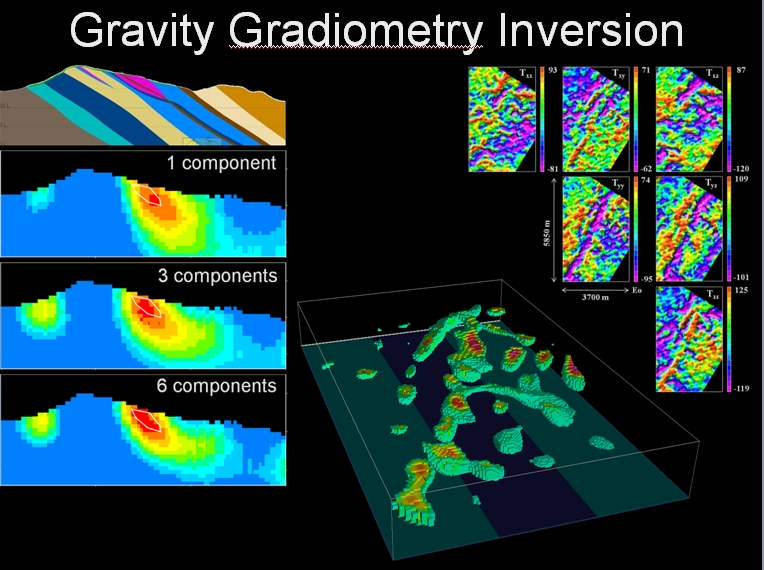
\includegraphics[width=0.95\PosterColumnTwoTextWidth{}]{YauguoExample}
    \end{figure}

    \vspace{1cm}
    It is easy to include figures! %
    Make sure you do not have odd edge artifacts like this one has. %
    Because the image can be re-sized, do not include text directly on your figures. %
    Instead, place the text on afterwards in \TeX{}.

  \end{minipage}
\end{textblock*}

% Column three text block dimensions
\newcommand{\PosterColumnThreeTextLeft}{\dimexpr (\PosterColumnThreeLeft + \PosterTextMarginSize)\relax}
\newcommand{\PosterColumnThreeTextWidth}{\dimexpr (\PosterColumnThreeWidth - 2\PosterTextMarginSize)\relax}
\newcommand{\PosterColumnThreeTextTop}{\dimexpr (\PosterColumnThreeTop + \PosterTextMarginSize)\relax}
\newcommand{\PosterColumnThreeTextHeight}{\dimexpr (\PosterColumnThreeHeight - 2\PosterTextMarginSize)\relax}

% Column three text 
\begin{textblock*}{\PosterColumnThreeTextWidth{}}(\PosterColumnThreeTextLeft{},\PosterColumnThreeTextTop{})
  \textblockcolor{ZeroColor}
  \begin{minipage}[t][\PosterColumnThreeTextHeight{}][t]{\PosterColumnThreeTextWidth{}}
    \vspace{5mm}
    % Discussion section
    \begin{center}
      \large
      \textbf{Discussion}
    \end{center}

    \vspace{5mm}
    \small
    Explain what you have done here. %
    Successes. Failures. Open questions?

    \vspace{50cm}
    \PosterColumnHorizontalBar{}
    % Bibliography section
    \begin{center}
      \large
      \textbf{References}
    \end{center}

    \renewcommand*{\bibfont}{\small}
    \printbibliography

  \end{minipage}
\end{textblock*}


\end{document}
